%%%%%%%%%%%%%%%%%%%%%%%%%%%%%%%%%%%%%%%%%%%%%%%%%%%%%%%%%%%%%%%%%%%%%%%%%%%%%%%
%
% Filename: ira-analysis.tex
% Author:   David Oniani
% Modified: October 17, 2019
%  _         _____   __  __
% | |    __ |_   _|__\ \/ /
% | |   / _` || |/ _ \\  /
% | |__| (_| || |  __//  \
% |_____\__,_||_|\___/_/\_\
%
%%%%%%%%%%%%%%%%%%%%%%%%%%%%%%%%%%%%%%%%%%%%%%%%%%%%%%%%%%%%%%%%%%%%%%%%%%%%%%%

%%%%%%%%%%%%%%%%%%%%%%%%%%%%%%%%%%%%%%%%%%%%%%%%%%%%%%%%%%%%%%%%%%%%%%%%%%%%%%%
% Document definition
%%%%%%%%%%%%%%%%%%%%%%%%%%%%%%%%%%%%%%%%%%%%%%%%%%%%%%%%%%%%%%%%%%%%%%%%%%%%%%%

\documentclass[12pt]{article}

%%%%%%%%%%%%%%%%%%%%%%%%%%%%%%%%%%%%%%%%%%%%%%%%%%%%%%%%%%%%%%%%%%%%%%%%%%%%%%%
% Packages and related settings
%%%%%%%%%%%%%%%%%%%%%%%%%%%%%%%%%%%%%%%%%%%%%%%%%%%%%%%%%%%%%%%%%%%%%%%%%%%%%%%

% Global, document-wide settings
\usepackage[margin=1in]{geometry}
\usepackage[utf8]{inputenc}
\usepackage[english]{babel}

% Bibliography and references
\usepackage[backend=biber]{biblatex}
\addbibresource{$BIB}

% Math and alignment
\usepackage{multicol}
\usepackage{bookmark}
\usepackage{adjustbox}
\usepackage{braket}
\usepackage{mathtools}
\usepackage{amsmath}
\usepackage{amssymb}
\usepackage{amsthm}
\usepackage{amsfonts}
\usepackage{algorithmic}

% Graphics
\usepackage{pgfplots}
\pgfplotsset{compat=1.16}
\usepackage{tikz}
\usetikzlibrary{cd, arrows, decorations.markings}
\usepackage{graphicx}
\usepackage{rotating}
\usepackage{pst-solides3d}
\usepackage{xcolor}

% Fancy stuff
\usepackage{fancyhdr}
\usepackage{tocloft}
\usepackage{caption}
\usepackage{soul}
\usepackage{textcomp}
\usepackage{wasysym}
\usepackage[cache=false]{minted}
\usepackage{csquotes}
\usepackage{hyperref}
\usepackage{subfig}

%%%%%%%%%%%%%%%%%%%%%%%%%%%%%%%%%%%%%%%%%%%%%%%%%%%%%%%%%%%%%%%%%%%%%%%%%%%%%%%
% Mathematican operations and operators
%%%%%%%%%%%%%%%%%%%%%%%%%%%%%%%%%%%%%%%%%%%%%%%%%%%%%%%%%%%%%%%%%%%%%%%%%%%%%%%

% Sets and related operators
\newcommand{\nats}{\mathbb{N}}                   % Natural numbers
\newcommand{\pnats}{\mathbb{N}^+}                % Positive natural numbers

\newcommand{\ints}{\mathbb{Z}}                   % Integers
\newcommand{\pints}{\mathbb{Z}^+}                % Positive integers
\newcommand{\nints}{\mathbb{Z}^-}                % Negative integers

\newcommand{\rats}{\mathbb{Q}}                   % Rational numbers
\newcommand{\prats}{\mathbb{Q}^+}                % Positive rational numbers
\newcommand{\nrats}{\mathbb{Q}^-}                % Negative rational numbers

\newcommand{\reals}{\mathbb{R}}                  % Real numbers
\newcommand{\preals}{\mathbb{R}^+}               % Positive real numbers
\newcommand{\nreals}{\mathbb{R}^-}               % Negative real numbers

\newcommand{\irrats}{\mathbb{I}}                 % Irrational numbers

\newcommand{\pset}{\mathcal{P}}                  % Powerset
\newcommand{\card}{\abs}                         % Cardinality
\newcommand{\topology}{\mathcal{T}}              % Topology
\newcommand{\basis}{\mathcal{B}}                 % Basis
\newcommand{\oldemptyset}{\emptyset}             % Old empty set
\renewcommand{\emptyset}{\varnothing}            % New and nice empty set

% Other operators
\DeclarePairedDelimiter\abs{\lvert}{\rvert}      % Absolute value
\DeclarePairedDelimiter\ceil{\lceil}{\rceil}     % Ceiling
\DeclarePairedDelimiter\floor{\lfloor}{\rfloor}  % Floor

%%%%%%%%%%%%%%%%%%%%%%%%%%%%%%%%%%%%%%%%%%%%%%%%%%%%%%%%%%%%%%%%%%%%%%%%%%%%%%%
% Command definitions and redefinitions
%%%%%%%%%%%%%%%%%%%%%%%%%%%%%%%%%%%%%%%%%%%%%%%%%%%%%%%%%%%%%%%%%%%%%%%%%%%%%%%

% New commands
\newcommand{\rarr}{\rightarrow}                        % Leftarrow
\newcommand{\larr}{\leftarrow}                         % Rightarrow
\newcommand\und[1]{\underline{\smash{#1}}}             % Nice-looking underline

% Renewed commands
\renewcommand{\headrulewidth}{0.5pt}                   % Header rule width
\renewcommand{\footrulewidth}{0pt}                     % Footer rule width
\renewcommand{\baselinestretch}{1.5}                   % Line spacing is 1.5
\renewcommand{\cftsecleader}{\cftdotfill{\cftdotsep}}  % Dots for ToC sections

% Rename "Contents" to "Table of Contents"
\addto\captionsenglish{% Replace "english" with the language used
  \renewcommand{\contentsname}%
    {\textbf{Table of Contents}}}%

% Filling the space for centering the title of the table of contents
\renewcommand{\cfttoctitlefont}{\hspace*{\fill}\Large}
\renewcommand{\cftaftertoctitle}{\hspace*{\fill}}

%%%%%%%%%%%%%%%%%%%%%%%%%%%%%%%%%%%%%%%%%%%%%%%%%%%%%%%%%%%%%%%%%%%%%%%%%%%%%%%
% Miscellaneous
%%%%%%%%%%%%%%%%%%%%%%%%%%%%%%%%%%%%%%%%%%%%%%%%%%%%%%%%%%%%%%%%%%%%%%%%%%%%%%%

% Setting stuff
\setlength{\parindent}{0pt}  % Remove indentations from paragraphs
\frenchspacing               % Get rid of large spaces after dots
\pagestyle{fancy}            % This allows to do fancy headers and footers
\fancyhf{}                   % No additional page numbering (or other stuff)
\cfoot{\thepage}             % Display page number at the bottom, in the center

% PDF information and nice-looking urls
\hypersetup{%
  pdfauthor  = {David Oniani},
  pdftitle   = {Textual and Statistical Analysis of Russian IRA Facebook Posts},
  pdfsubject = {Statistics, Authorship Attribution, Visual Persuasion},
  colorlinks = true,
  linkcolor  = {blue!50!black},
  citecolor  = {blue!50!black},
  urlcolor   = {blue!50!black}
}

% Put a centered header of a footnote size on the top of each page
\chead{\footnotesize{\MakeUppercase{Textual and Statistical Analysis of Russian IRA Facebook Posts}}}

% Definition environment
\theoremstyle{definition}
\newtheorem*{definition}{Definition}

%%%%%%%%%%%%%%%%%%%%%%%%%%%%%%%%%%%%%%%%%%%%%%%%%%%%%%%%%%%%%%%%%%%%%%%%%%%%%%%
% Author(s), title, and date
%%%%%%%%%%%%%%%%%%%%%%%%%%%%%%%%%%%%%%%%%%%%%%%%%%%%%%%%%%%%%%%%%%%%%%%%%%%%%%%

% Author(s)
\author{David Oniani\\
        Luther College\\
        \href{mailto:oniada01@luther.edu}{oniada01@luther.edu}}

% Title
\title{\textbf{Textual and Statistical Analysis of Russian IRA Facebook Posts}\\
      \small \textsuperscript{*}The paper is written in the scope of a student-faculty collaborative\\
                                summer research with professor Richard K. Merritt.}

% Date
\date{Month Day, Year}

%%%%%%%%%%%%%%%%%%%%%%%%%%%%%%%%%%%%%%%%%%%%%%%%%%%%%%%%%%%%%%%%%%%%%%%%%%%%%%%
% Beginning of the document
%%%%%%%%%%%%%%%%%%%%%%%%%%%%%%%%%%%%%%%%%%%%%%%%%%%%%%%%%%%%%%%%%%%%%%%%%%%%%%%

\begin{document}
\maketitle

%%%%%%%%%%%%%%%%%%%%%%%%%%%%%%%%%%%%%%%%%%%%%%%%%%%%%%%%%%%%%%%%%%%%%%%%%%%%%%%
% Abstract
%%%%%%%%%%%%%%%%%%%%%%%%%%%%%%%%%%%%%%%%%%%%%%%%%%%%%%%%%%%%%%%%%%%%%%%%%%%%%%%

\begin{abstract}
\addcontentsline{toc}{section}{Abstract}

\noindent The 2016 United States Presidential Election was targeted by an
unprecedented intelligence and influence campaign. Arising out of Russian
so-called Internet Research Agency (IRA), it sought to sow discord and attack
the fissures of the United States with the ultimate goal of swaying the
election results.~\cite{ira2016}~\cite{ira2016data} Recently, some of the
IRA-backed Facebook advertisements were released by The United States House
Permanent Select Committee on Intelligence. All of the advertisements are in
the PDF format. We have scraped the PDF files and present the results obtained
by both textual and statistical analysis of the above-mentioned data. Authorship
attribution and sentiment analysis tests were performed.~\footnote{Please note
that this paper does not discuss neither social, nor political implications of
these events, but attempts to explore the methods of persuasion that were
employed in this influence campaign.}~\cite{ira2016csvdata} We have also made
the data publicly available for other researchers and/or interested people in
a much nicer and easier-to-manipulate CSV format.
\end{abstract}

%%%%%%%%%%%%%%%%%%%%%%%%%%%%%%%%%%%%%%%%%%%%%%%%%%%%%%%%%%%%%%%%%%%%%%%%%%%%%%%
% Table of Contents
%%%%%%%%%%%%%%%%%%%%%%%%%%%%%%%%%%%%%%%%%%%%%%%%%%%%%%%%%%%%%%%%%%%%%%%%%%%%%%%

\newpage
\tableofcontents
\newpage

%%%%%%%%%%%%%%%%%%%%%%%%%%%%%%%%%%%%%%%%%%%%%%%%%%%%%%%%%%%%%%%%%%%%%%%%%%%%%%%
% Data and Preparation
%%%%%%%%%%%%%%%%%%%%%%%%%%%%%%%%%%%%%%%%%%%%%%%%%%%%%%%%%%%%%%%%%%%%%%%%%%%%%%%

\section*{\centering Data and Preparation}
\addcontentsline{toc}{section}{Data and Preparation}

The dataset was scraped from~\cite{ira2016data} more than 3500 Russian IRA
Facebook posts made publicly available in the PDF format by the House
Intelligence Committee. We used the free and open-source Python library
~\cite{pdftotext} \texttt{pdftotext} to scrape the data. Many CSV files were
formatted in a way that it was virtually impossible for \texttt{pdftotext} to
scrape it correctly. Because of this, we have manually reviewed most of the
CSV files for validity.~\cite{ira2016csvdata} All the CSV files have been made
publicly available. It is important to note that the dataset is just a sample
of a bigger dataset, and albeit less likely, might not be a good representatation
for the overall campaign.

%%%%%%%%%%%%%%%%%%%%%%%%%%%%%%%%%%%%%%%%%%%%%%%%%%%%%%%%%%%%%%%%%%%%%%%%%%%%%%%
% Textual Analysis
%%%%%%%%%%%%%%%%%%%%%%%%%%%%%%%%%%%%%%%%%%%%%%%%%%%%%%%%%%%%%%%%%%%%%%%%%%%%%%%

\section*{\centering Textual Analysis}
\addcontentsline{toc}{section}{Textual Analysis}

%%%%%%%%%%%%%%%%%%%%%%%%%%%%%%%%%%%%%%%%%%%%%%%%%%%%%%%%%%%%%%%%%%%%%%%%%%%%%%%
% Common Words
%%%%%%%%%%%%%%%%%%%%%%%%%%%%%%%%%%%%%%%%%%%%%%%%%%%%%%%%%%%%%%%%%%%%%%%%%%%%%%%

\subsection*{\centering Common Words}
\addcontentsline{toc}{subsection}{Common Words}

Among the targeting strategies utilized by this influence campaign, one of the
rather noticeable ones was exploiting the internal fissures of the United States
by realizing social, political, historical background of the country.

\bigskip

Three most commonly used words in the campaign were black, police, and people.
~\footnote{The list of all eliminated words is provided at\\
\url{https://github.com/oniani/ira-analysis/blob/master/eliminated-words.txt}.}
Below is the barchart showing top 25 most commonly used words after eliminating
linking verbs, prepositions, pronouns, and some other (non-relevant) words.

\begin{figure}[H]
\centering
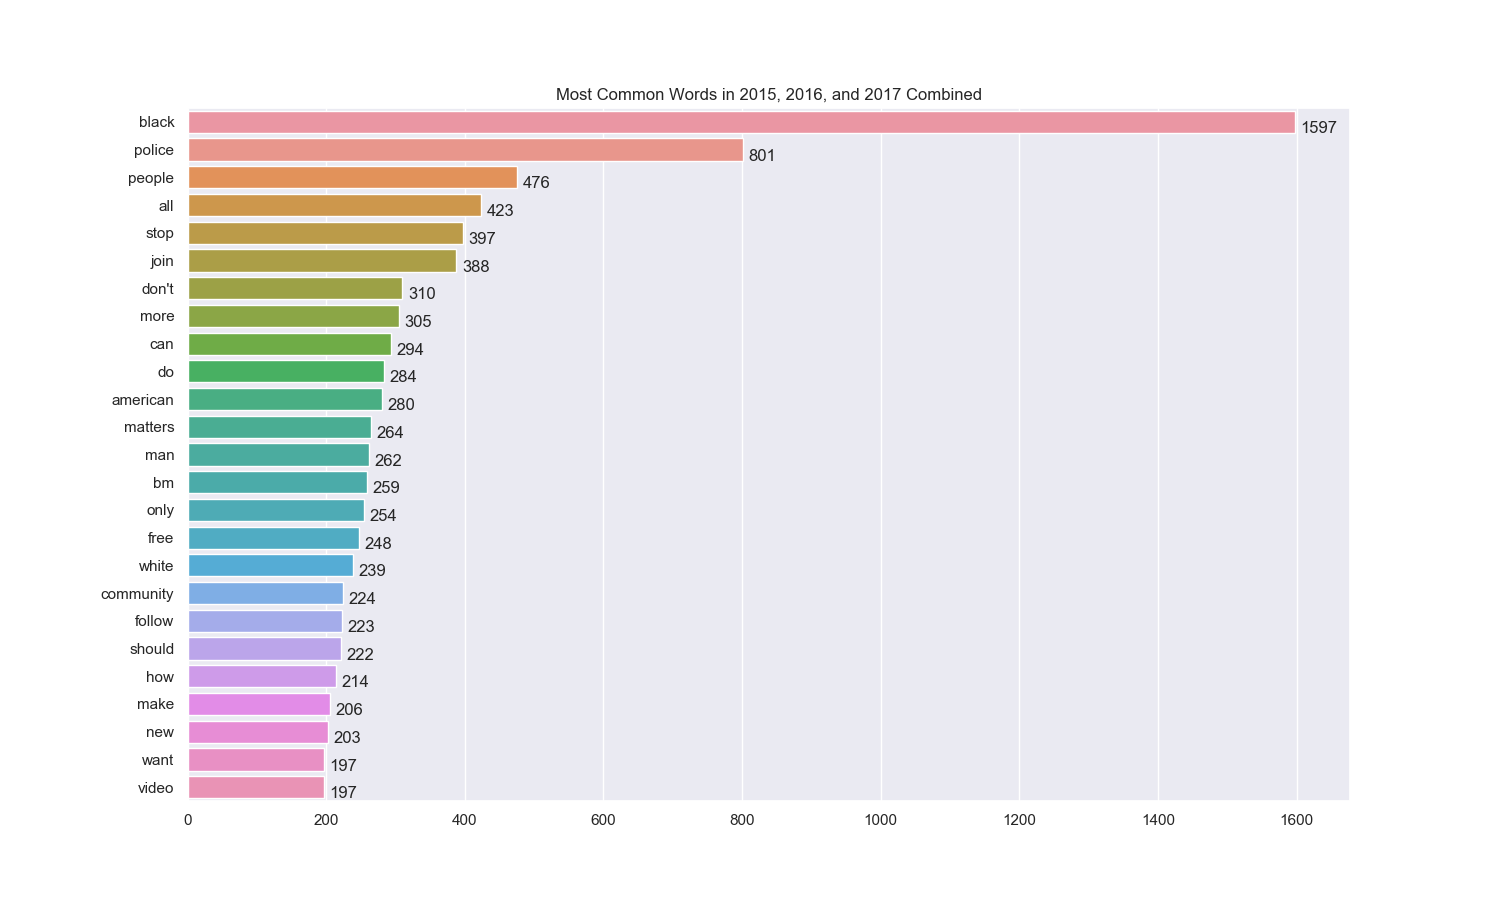
\includegraphics[width=\columnwidth]{./image/barchart-plots/barchart_word_counts.png}
\caption*{Most common words in 2015, 2016, and 2017 combined.}
\end{figure}

%%%%%%%%%%%%%%%%%%%%%%%%%%%%%%%%%%%%%%%%%%%%%%%%%%%%%%%%%%%%%%%%%%%%%%%%%%%%%%%
% Sentiment Analysis
%%%%%%%%%%%%%%%%%%%%%%%%%%%%%%%%%%%%%%%%%%%%%%%%%%%%%%%%%%%%%%%%%%%%%%%%%%%%%%%

\subsubsection*{\centering Sentiment Analysis}
\addcontentsline{toc}{subsection}{Sentiment Analysis}
For the sentiment analysis purposes, we used \texttt{python}'s \texttt{TextBlob}
library. Suprisingly, out of all Facebook posts with \texttt{Ad Text}, 1643 were
positive, 900 negative, and 933 neutral leaving the overall tone of the posts
positive. Yet, the statistical significance of this claim is rather questionable
as the polarity levels were always near zero. Such low polarity level, however,
demonstrates a highly intelligent design of posts maximizing efficiency of
persuading targeted audience.

\bigskip

As the \texttt{Ad Text}s did not give us any strong proofs, we looked at the
negativity levels across all three years and found a consistent trend.

\begin{figure}[H]
\centering
\begin{tabular}{|p{3cm}|p{3cm}|p{3cm}|p{3cm}|p{3cm}|}
 \hline
 Subjectivity & Year 2015 & Year 2016 & Year 2017 & 2016 (\%)\\
 \hline
 1.0  & 154 & 562 & 176 & 63.004\\
 \hline
 0.75 & 150 & 547 & 169 & 63.164\\
 \hline
 0.5  & 123 & 405 & 120 & 62.500\\
 \hline
 0.25 & 15  & 81  & 22  & 68.644\\
 \hline
 0.15 & 5   & 33  & 10  & 68.750\\
 \hline
 0.1  & 2   & 11  & 6   & 57.895\\
 \hline
 0.05 & 1   & 5   & 2   & 62.500\\
 \hline
\end{tabular}
\caption*{Analyzing Negativity}
\end{figure}

\bigskip

Notice that for any given year and at any subjectivity level, year 2016 is
consistently comprising around 60\% of all posts. The year of the Presidentianl
Election was rather negative.

%%%%%%%%%%%%%%%%%%%%%%%%%%%%%%%%%%%%%%%%%%%%%%%%%%%%%%%%%%%%%%%%%%%%%%%%%%%%%%%
% Authorship Attribution
%%%%%%%%%%%%%%%%%%%%%%%%%%%%%%%%%%%%%%%%%%%%%%%%%%%%%%%%%%%%%%%%%%%%%%%%%%%%%%%

\subsubsection*{\centering Authorship Attribution}
\addcontentsline{toc}{subsection}{Authorship Attribution}

Since all of these posts were issued by the same organization/entity, it was
interesting to see if there are some common patterns between the Facebook ads
of 2015, 2016, 2017. For this exact reason, we have performed authorship
attribution tests by implementing~\cite{koppel11} the paper by Koppel et.~al.

\bigskip

We have performed 3 authorship attribution tests:

\begin{enumerate}
  \item Assuming that the author of the Facebook posts of 2016 and 2017 was the
        same and checking accuracy for the author of 2015.

  \item Assuming that the author of the Facebook posts of 2015 and 2017 was the
        same and checking accuracy for the author of 2016.

  \item Assuming that the author of the Facebook posts of 2015 and 2016 was the
        same and checking accuracy for the author of 2017.
\end{enumerate}

In all three cases, we had to merge some of the data to achieve the required
minimum text length of 500 words.~\footnote{Note that because of randomization,
texts were somewhat scrambled and are not available in any format. That said,
one can easily redo the authorship attribution with similar accuracy using
the algorithm which already implemented and resides in the GitHub repository,
\url{https://github.com/oniani/ira-analysis/tree/master/koppel11}.}
This was done using randomization to avoid bias.~\footnote{Results JSON:
\url{https://github.com/oniani/ira-analysis/tree/master/koppel11/results}}
Results are available in the form of JSON files formatted in the manner shown
below.

\begin{figure}[H]
\begin{minted}[frame=single, linenos=true, tabsize=2]{js}
{
  "answers": [
    {
      "unknown_text": "2015-unknown1.txt",
      "author": "candidate2016",
      "score": 0.58
    },
    ...
    {
      "unknown_text": "2015-unknown56.txt",
      "author": "candidate2016",
      "score": 0.76
    }
  ]
}
\end{minted}
\caption*{JSON example}
\end{figure}

The first answer tells us that the unknown text was written in year 2015, and
that there is 58\% chance that it was written by the author of Facebook posts
of 2016. The last answer shows that there is 0.76\% chance that the given
text was authored by the entity who wrote the posts in year 2016.

\bigskip

Below are the results obtained after performing all three above-mentioned
authorship attribution tasks.

\begin{figure}[H]
\centering
\begin{tabular}{|p{8cm}|p{8cm}|}
 \hline
 \multicolumn{2}{|c|}{Average Accuracy}\\
 \hline
 Years & Similarity (\%)\\
 \hline
 2016 and 2017 & 72.509\% (similarity to 2015)\\
 \hline
 2015 and 2017 & 68.516\% (similarity to 2016)\\
 \hline
 2015 and 2016 & 62.392\% (similarity to 2017)\\
 \hline
 Average (2015, 2016, and 2017) & 67.806\%\\
 \hline
\end{tabular}
\caption*{Average Accuracy}
\end{figure}

\bigskip

%%%%%%%%%%%%%%%%%%%%%%%%%%%%%%%%%%%%%%%%%%%%%%%%%%%%%%%%%%%%%%%%%%%%%%%%%%%%%%%
% Statistical Analysis
%%%%%%%%%%%%%%%%%%%%%%%%%%%%%%%%%%%%%%%%%%%%%%%%%%%%%%%%%%%%%%%%%%%%%%%%%%%%%%%

\section*{\centering Statistical Analysis}
\addcontentsline{toc}{section}{Statistical Analysis}

%%%%%%%%%%%%%%%%%%%%%%%%%%%%%%%%%%%%%%%%%%%%%%%%%%%%%%%%%%%%%%%%%%%%%%%%%%%%%%%
% General Statistics
%%%%%%%%%%%%%%%%%%%%%%%%%%%%%%%%%%%%%%%%%%%%%%%%%%%%%%%%%%%%%%%%%%%%%%%%%%%%%%%

\subsection*{\centering General Statistics}
\addcontentsline{toc}{subsection}{General Statistics}
The distribution of posts over all three years shows a bimodal distribution
with two peaks in quarters 2 and 4 of year 2016. Given the fact that the US
Presidential Election was held in the fourth quarter of 2016, it is surprising
that the number of posts in the second quarter exceeded that of the fourth
quarter.

\begin{figure}[H]
\centering
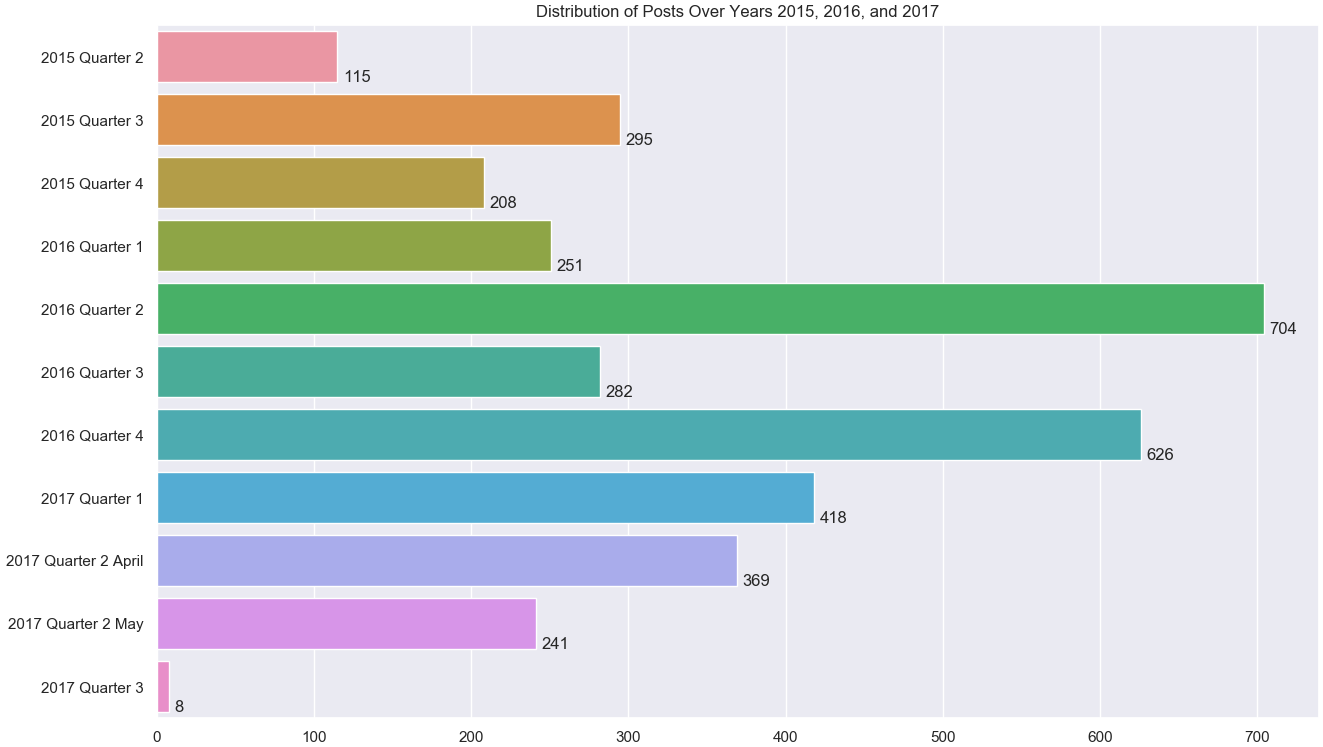
\includegraphics[width=0.75\columnwidth]{./image/barchart-plots/barchart_distribution_of_posts.png}
\caption*{Distribution of Posts Over Years 2015, 2016, and 2017.}
\end{figure}

As for ad spendings, the fourth quarter of 2016 exceeds that of any quarter,
with second quarter coming next. Interestingly, most of ads were paid in the
Russian currency (ruble) with two exceptions in 2016 quarter 3 and 2017 quarter
1 when IRA spent \$74.000 and \$35.330 respectively.

\begin{figure}[H]
\centering
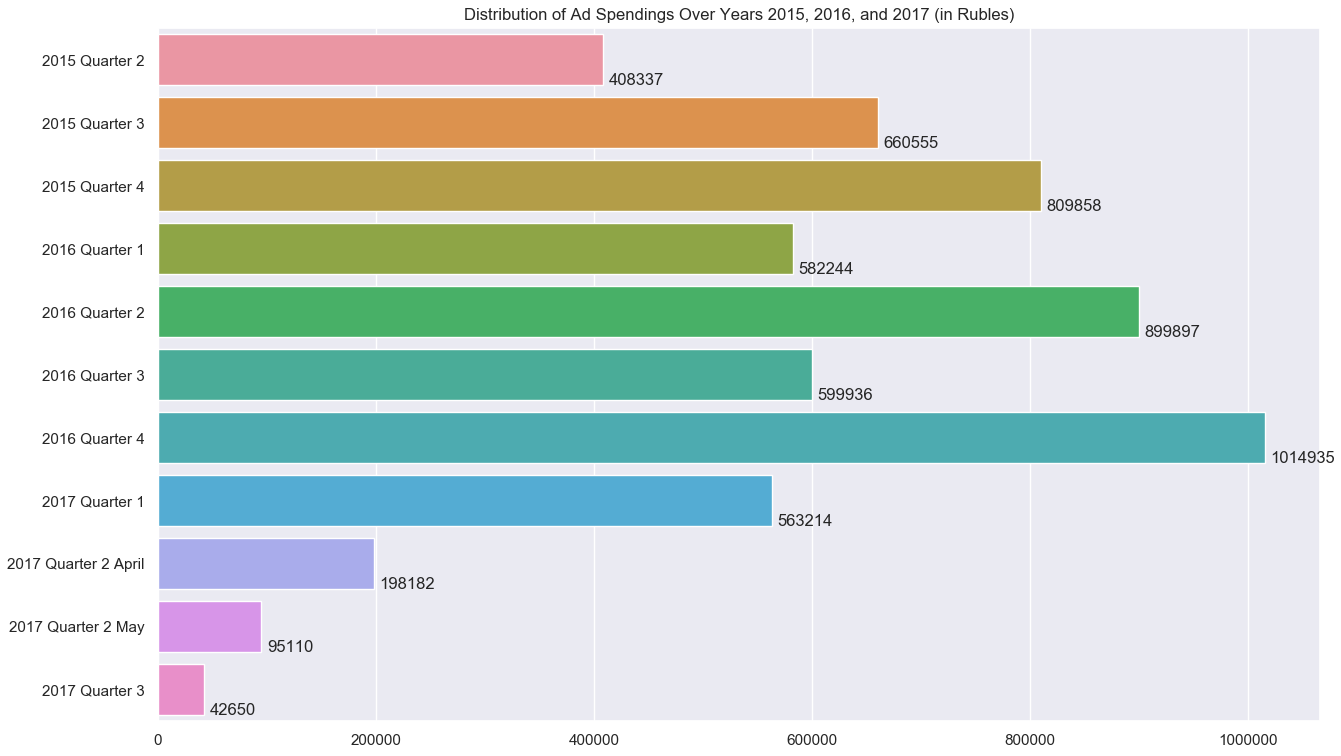
\includegraphics[width=0.75\columnwidth]{./image/barchart-plots/barchart_ad_spend_RU_distribution.png}
\caption*{Distribution of Ad Spendings Over Years 2015, 2016, and 2017 (in rubles).}
\end{figure}

Furthermore, 99.8\% of all paid ads across all years were paid in rubles.
Below is the chart showing the number of posts based on a currency.

\begin{center}
\begin{tabular}{|p{3cm}|p{3cm}|}
 \hline
 Currency & \text{Total (All Years)}\\
 \hline
 RUB  & 2549\\
 \hline
 USD  & 5\\
 \hline
 None & 787\\
 \hline
 0    & 176\\
 \hline
\end{tabular}
\end{center}

\bigskip

As the information for the reader, the Russian ruble is used only in Russia,
Belarus, and two regions of Georgia, which are considered by Russia as partially
recognized states of Abkhazia and South Ossetia.

%%%%%%%%%%%%%%%%%%%%%%%%%%%%%%%%%%%%%%%%%%%%%%%%%%%%%%%%%%%%%%%%%%%%%%%%%%%%%%%
% Regression Analysis
%%%%%%%%%%%%%%%%%%%%%%%%%%%%%%%%%%%%%%%%%%%%%%%%%%%%%%%%%%%%%%%%%%%%%%%%%%%%%%%

\subsection*{\centering Hypothesis Testing}
\addcontentsline{toc}{subsection}{Hypothesis Testing}

\begin{figure}[H]
\centering
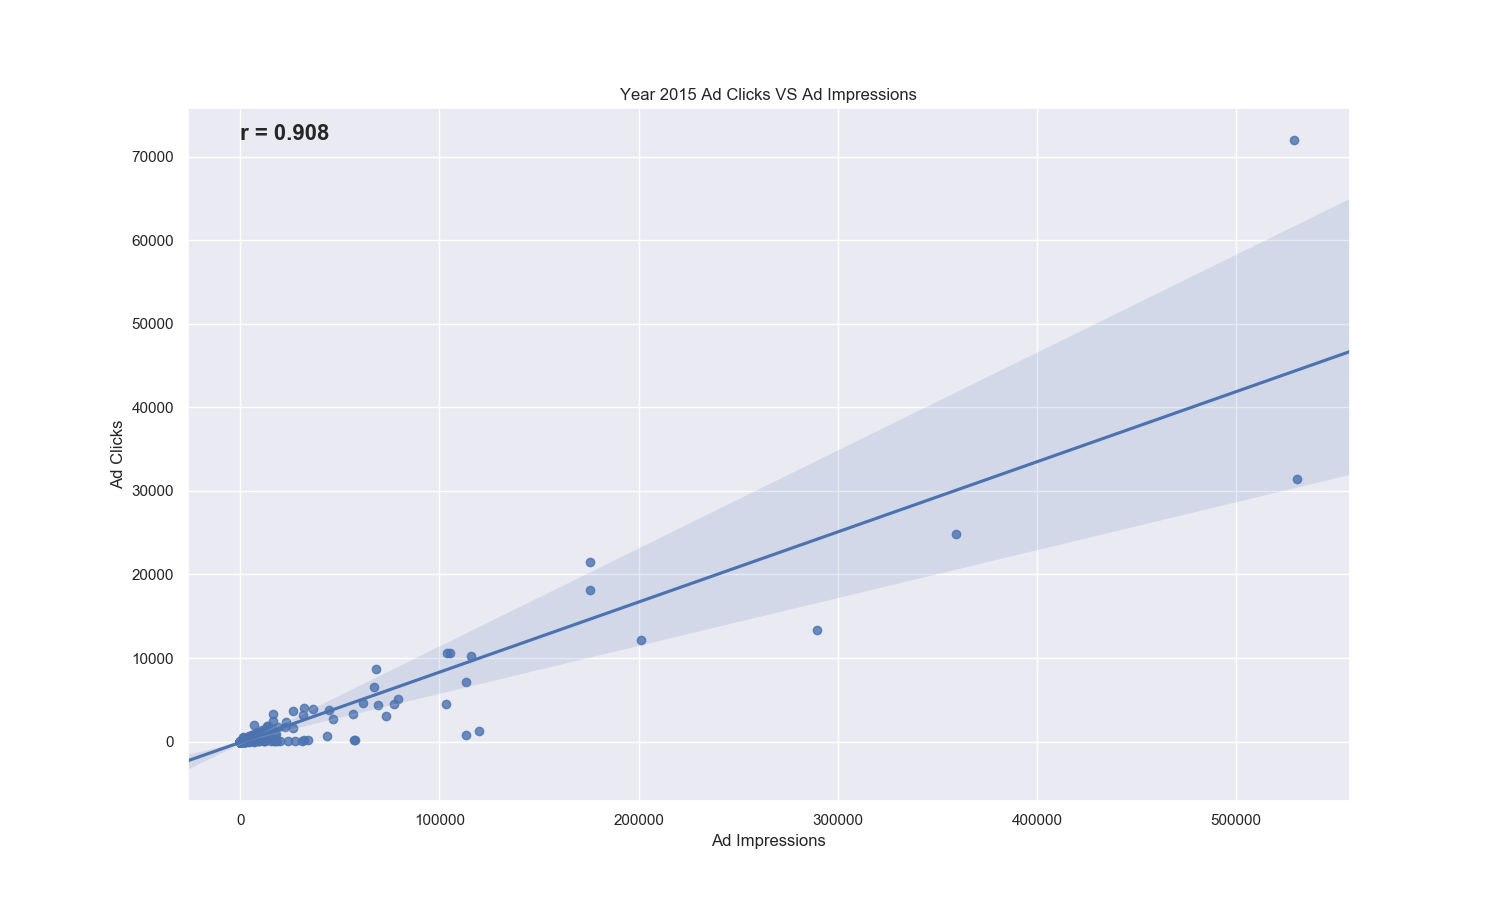
\includegraphics[width=\columnwidth]{./image/regression-plots/ad-clicks-vs-ad-impressions/year-2015-ad-clicks-vs-ad-impressions.png}
\caption*{Year 2016 Ad Clicks VS Ad Impressions.}
\end{figure}

%%%%%%%%%%%%%%%%%%%%%%%%%%%%%%%%%%%%%%%%%%%%%%%%%%%%%%%%%%%%%%%%%%%%%%%%%%%%%%%
% Regression Analysis
%%%%%%%%%%%%%%%%%%%%%%%%%%%%%%%%%%%%%%%%%%%%%%%%%%%%%%%%%%%%%%%%%%%%%%%%%%%%%%%

\subsection*{\centering Regression Analysis}
\addcontentsline{toc}{subsection}{Regression Analysis}

For our first hypothesis test, we would like to determine if there is a
statistically significant relationship between two quantitative variables:
the length of advertisement text and the money paid for it.

\bigskip

Determinining whether there is a statistically significant between these two
variables will give us an idea if there was some kind of priority attached
to posts, depending on the length.

\bigskip

For this task, we use a linear regression approach. Note that we perform the
test only on the ads paid in rubles, the primary reason being not having enough
data points for USD (only 5 values).

\bigskip

$H_0$: There is a statistically significant relationship between the amount
of money paid and the length of the text in the advertisement.

\bigskip

$H_0$: There is no statistically significant relationship between the amount
of money paid and the length of the text in the advertisement.

\begin{figure}
  \centering
  \subfloat[Money Spent VS Ad Spend Length]{{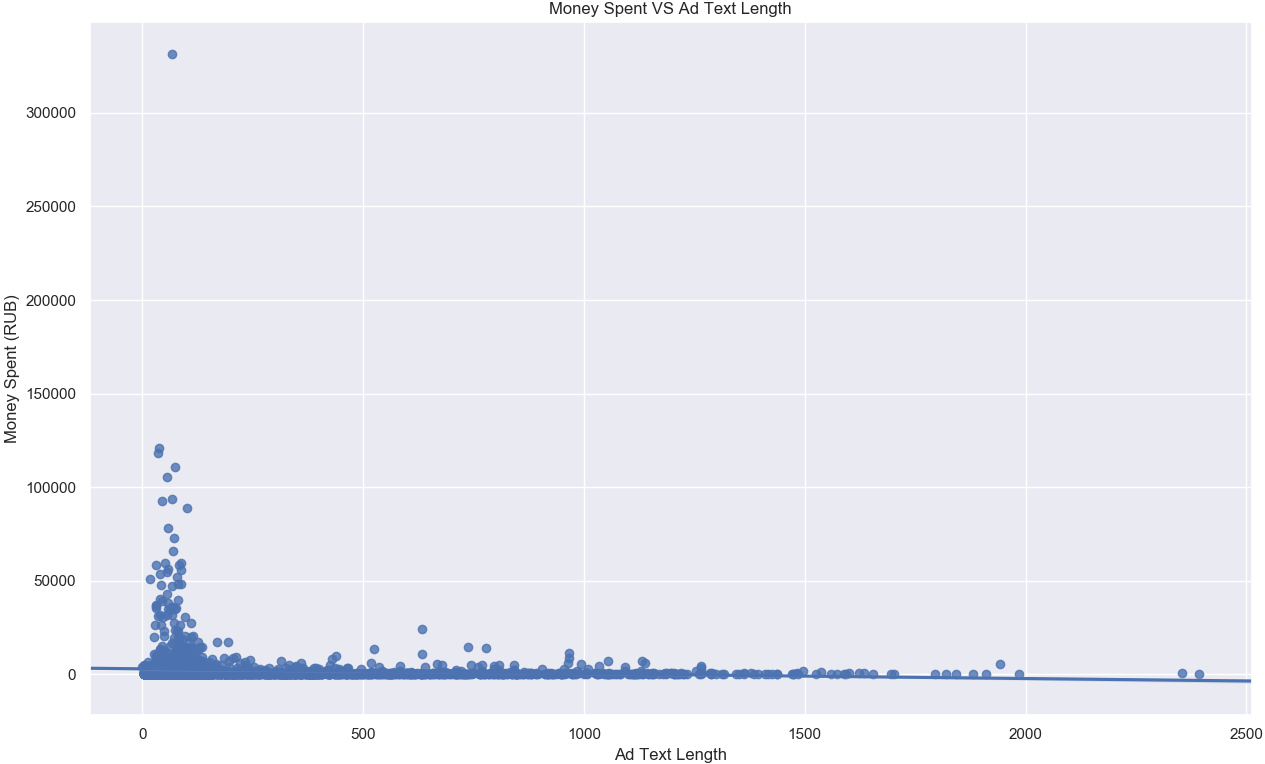
\includegraphics[width=8cm]{./image/regression-plots/ad_spend_text_length_regression.png}}}
  \hfill
  \subfloat[Log Money Spent VS Log Ad Spend Length]{{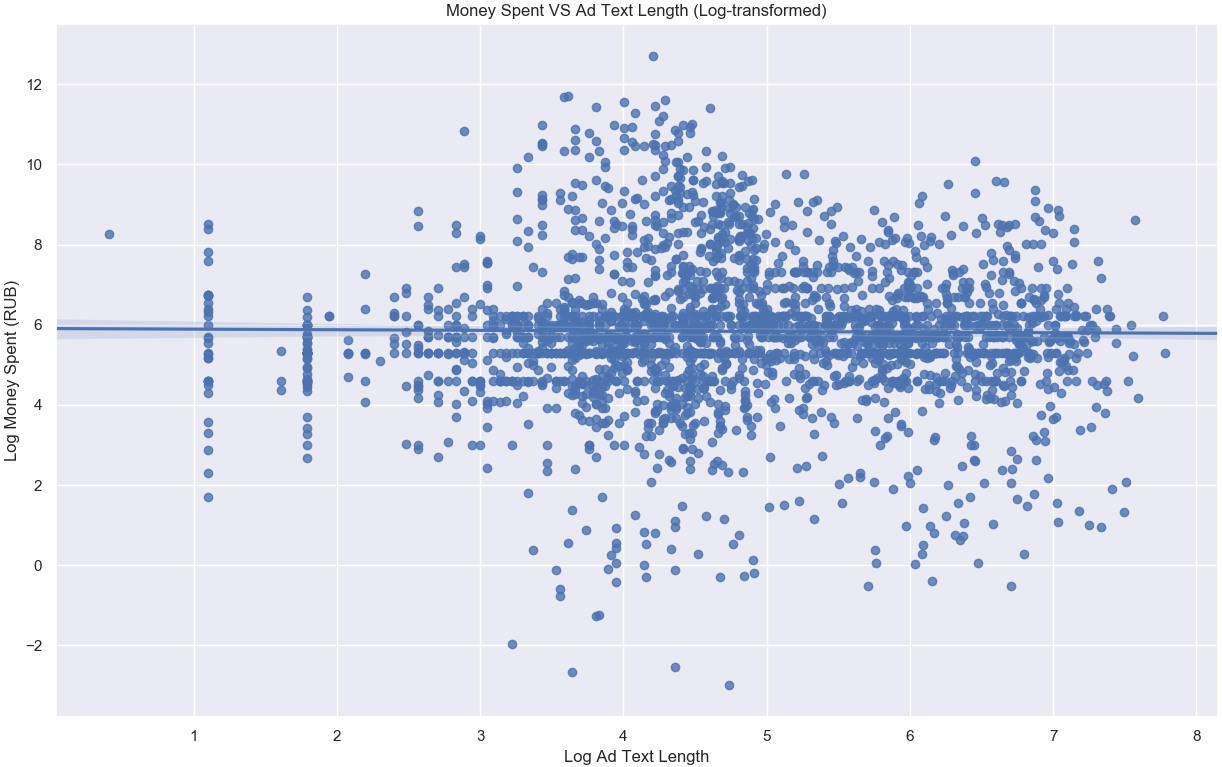
\includegraphics[width=8cm]{./image/regression-plots/ad_spend_text_length_regression_log_transform.png}}}
  \caption*{Simple VS Log-transformed}
  \label{fig:example}
\end{figure}

\bigskip

\begin{center}
\begin{tabular}{|p{3cm}|p{3cm}|}
 \hline
 \multicolumn{2}{|c|}{RUB (Without Log Transform)}\\
 \hline
 Slope          & -2.594\\
 \hline
 Intercept      & 2980.780\\
 \hline
 R-squared      & 0.007\\
 \hline
 P-value        & $3.680 * 10^{-5}$\\
 \hline
 Standard Error & 0.627\\
 \hline
\end{tabular}
\qquad
\begin{tabular}{|p{3cm}|p{3cm}|}
 \hline
 \multicolumn{2}{|c|}{RUB (With Log Transform)}\\
 \hline
 Slope          & -0.015\\
 \hline
 Intercept      & 5.904\\
 \hline
 R-squared      & 0.0001\\
 \hline
 P-value        & $0.594 * 10^{-5}$\\
 \hline
 Standard Error & 0.028\\
 \hline
\end{tabular}
\end{center}

\bigskip

From the chart above, we see the R-squared value of \$0.007, which tells us
that only 0.7\% of variation in the money paid for advertisements is explained
by the number of words. Standard error is 0.627 which is very small compared
to the intercept whose value is 2980.780 (RUB). This tells us that the error
in our estimates is really small. The p-value equals $3.680 * 10^{-5}$ which
is a lot smaller than $0.05$ and makes the conclusion statistically significant.
Therefore, we accept the null and reject the alternative conclude that there
is no statistically relationship between the amount of money paid and the
number of words in the advertisement.

\bigskip

Even after performing a log-transform, the results are still bleak.

\bigskip

Although having no relationship is usually not a desired result, in our case,
we conclue that posts were designed in a rather smart manner, with no
noticeable priorities attached, depending on the number of words in the post.

%%%%%%%%%%%%%%%%%%%%%%%%%%%%%%%%%%%%%%%%%%%%%%%%%%%%%%%%%%%%%%%%%%%%%%%%%%%%%%%
% Conclusions
%%%%%%%%%%%%%%%%%%%%%%%%%%%%%%%%%%%%%%%%%%%%%%%%%%%%%%%%%%%%%%%%%%%%%%%%%%%%%%%

\section*{\centering Conclusions}
\addcontentsline{toc}{section}{Conclusions}

Lorem ipsum dolor sit amet, consectetur adipiscing elit.
Aenean porta purus et sem gravida rutrum.
Maecenas blandit nulla ac luctus tempus.
Nam finibus posuere ante, et lacinia massa vestibulum sit amet.
Nulla velit arcu, efficitur quis turpis nec, sollicitudin lobortis nisi.
Vivamus ut diam ut eros faucibus fringilla.
Suspendisse pellentesque magna nec velit tristique sollicitudin.
Morbi ultrices nec augue et molestie.
Nam sapien ante, ullamcorper elementum convallis id, faucibus in lectus.
Fusce pellentesque mollis velit efficitur porta.
Sed finibus ligula quam, et lacinia velit posuere auctor.
Donec ligula lorem, dictum nec lectus in, vehicula tincidunt massa.
In hac habitasse platea dictumst.

%%%%%%%%%%%%%%%%%%%%%%%%%%%%%%%%%%%%%%%%%%%%%%%%%%%%%%%%%%%%%%%%%%%%%%%%%%%%%%%
% Bibliography and References
%%%%%%%%%%%%%%%%%%%%%%%%%%%%%%%%%%%%%%%%%%%%%%%%%%%%%%%%%%%%%%%%%%%%%%%%%%%%%%%

\newpage

\begin{center}
\printbibliography[heading=bibintoc]
\end{center}

%%%%%%%%%%%%%%%%%%%%%%%%%%%%%%%%%%%%%%%%%%%%%%%%%%%%%%%%%%%%%%%%%%%%%%%%%%%%%%%
% The end of the document
%%%%%%%%%%%%%%%%%%%%%%%%%%%%%%%%%%%%%%%%%%%%%%%%%%%%%%%%%%%%%%%%%%%%%%%%%%%%%%%

\end{document}
